% Options for packages loaded elsewhere
\PassOptionsToPackage{unicode}{hyperref}
\PassOptionsToPackage{hyphens}{url}
\PassOptionsToPackage{dvipsnames,svgnames,x11names}{xcolor}
%
\documentclass[
  11pt,
]{article}
\title{Breast Cancer Wisconsin (Diagnostic)}
\author{L. Favero}
\date{}

\usepackage{amsmath,amssymb}
\usepackage{lmodern}
\usepackage{iftex}
\ifPDFTeX
  \usepackage[T1]{fontenc}
  \usepackage[utf8]{inputenc}
  \usepackage{textcomp} % provide euro and other symbols
\else % if luatex or xetex
  \usepackage{unicode-math}
  \defaultfontfeatures{Scale=MatchLowercase}
  \defaultfontfeatures[\rmfamily]{Ligatures=TeX,Scale=1}
\fi
% Use upquote if available, for straight quotes in verbatim environments
\IfFileExists{upquote.sty}{\usepackage{upquote}}{}
\IfFileExists{microtype.sty}{% use microtype if available
  \usepackage[]{microtype}
  \UseMicrotypeSet[protrusion]{basicmath} % disable protrusion for tt fonts
}{}
\makeatletter
\@ifundefined{KOMAClassName}{% if non-KOMA class
  \IfFileExists{parskip.sty}{%
    \usepackage{parskip}
  }{% else
    \setlength{\parindent}{0pt}
    \setlength{\parskip}{6pt plus 2pt minus 1pt}}
}{% if KOMA class
  \KOMAoptions{parskip=half}}
\makeatother
\usepackage{xcolor}
\IfFileExists{xurl.sty}{\usepackage{xurl}}{} % add URL line breaks if available
\IfFileExists{bookmark.sty}{\usepackage{bookmark}}{\usepackage{hyperref}}
\hypersetup{
  pdftitle={Breast Cancer Wisconsin (Diagnostic)},
  pdfauthor={L. Favero},
  colorlinks=true,
  linkcolor={Maroon},
  filecolor={Maroon},
  citecolor={Blue},
  urlcolor={blue},
  pdfcreator={LaTeX via pandoc}}
\urlstyle{same} % disable monospaced font for URLs
\usepackage[margin=1in]{geometry}
\usepackage{color}
\usepackage{fancyvrb}
\newcommand{\VerbBar}{|}
\newcommand{\VERB}{\Verb[commandchars=\\\{\}]}
\DefineVerbatimEnvironment{Highlighting}{Verbatim}{commandchars=\\\{\}}
% Add ',fontsize=\small' for more characters per line
\usepackage{framed}
\definecolor{shadecolor}{RGB}{248,248,248}
\newenvironment{Shaded}{\begin{snugshade}}{\end{snugshade}}
\newcommand{\AlertTok}[1]{\textcolor[rgb]{0.94,0.16,0.16}{#1}}
\newcommand{\AnnotationTok}[1]{\textcolor[rgb]{0.56,0.35,0.01}{\textbf{\textit{#1}}}}
\newcommand{\AttributeTok}[1]{\textcolor[rgb]{0.77,0.63,0.00}{#1}}
\newcommand{\BaseNTok}[1]{\textcolor[rgb]{0.00,0.00,0.81}{#1}}
\newcommand{\BuiltInTok}[1]{#1}
\newcommand{\CharTok}[1]{\textcolor[rgb]{0.31,0.60,0.02}{#1}}
\newcommand{\CommentTok}[1]{\textcolor[rgb]{0.56,0.35,0.01}{\textit{#1}}}
\newcommand{\CommentVarTok}[1]{\textcolor[rgb]{0.56,0.35,0.01}{\textbf{\textit{#1}}}}
\newcommand{\ConstantTok}[1]{\textcolor[rgb]{0.00,0.00,0.00}{#1}}
\newcommand{\ControlFlowTok}[1]{\textcolor[rgb]{0.13,0.29,0.53}{\textbf{#1}}}
\newcommand{\DataTypeTok}[1]{\textcolor[rgb]{0.13,0.29,0.53}{#1}}
\newcommand{\DecValTok}[1]{\textcolor[rgb]{0.00,0.00,0.81}{#1}}
\newcommand{\DocumentationTok}[1]{\textcolor[rgb]{0.56,0.35,0.01}{\textbf{\textit{#1}}}}
\newcommand{\ErrorTok}[1]{\textcolor[rgb]{0.64,0.00,0.00}{\textbf{#1}}}
\newcommand{\ExtensionTok}[1]{#1}
\newcommand{\FloatTok}[1]{\textcolor[rgb]{0.00,0.00,0.81}{#1}}
\newcommand{\FunctionTok}[1]{\textcolor[rgb]{0.00,0.00,0.00}{#1}}
\newcommand{\ImportTok}[1]{#1}
\newcommand{\InformationTok}[1]{\textcolor[rgb]{0.56,0.35,0.01}{\textbf{\textit{#1}}}}
\newcommand{\KeywordTok}[1]{\textcolor[rgb]{0.13,0.29,0.53}{\textbf{#1}}}
\newcommand{\NormalTok}[1]{#1}
\newcommand{\OperatorTok}[1]{\textcolor[rgb]{0.81,0.36,0.00}{\textbf{#1}}}
\newcommand{\OtherTok}[1]{\textcolor[rgb]{0.56,0.35,0.01}{#1}}
\newcommand{\PreprocessorTok}[1]{\textcolor[rgb]{0.56,0.35,0.01}{\textit{#1}}}
\newcommand{\RegionMarkerTok}[1]{#1}
\newcommand{\SpecialCharTok}[1]{\textcolor[rgb]{0.00,0.00,0.00}{#1}}
\newcommand{\SpecialStringTok}[1]{\textcolor[rgb]{0.31,0.60,0.02}{#1}}
\newcommand{\StringTok}[1]{\textcolor[rgb]{0.31,0.60,0.02}{#1}}
\newcommand{\VariableTok}[1]{\textcolor[rgb]{0.00,0.00,0.00}{#1}}
\newcommand{\VerbatimStringTok}[1]{\textcolor[rgb]{0.31,0.60,0.02}{#1}}
\newcommand{\WarningTok}[1]{\textcolor[rgb]{0.56,0.35,0.01}{\textbf{\textit{#1}}}}
\usepackage{longtable,booktabs,array}
\usepackage{calc} % for calculating minipage widths
% Correct order of tables after \paragraph or \subparagraph
\usepackage{etoolbox}
\makeatletter
\patchcmd\longtable{\par}{\if@noskipsec\mbox{}\fi\par}{}{}
\makeatother
% Allow footnotes in longtable head/foot
\IfFileExists{footnotehyper.sty}{\usepackage{footnotehyper}}{\usepackage{footnote}}
\makesavenoteenv{longtable}
\usepackage{graphicx}
\makeatletter
\def\maxwidth{\ifdim\Gin@nat@width>\linewidth\linewidth\else\Gin@nat@width\fi}
\def\maxheight{\ifdim\Gin@nat@height>\textheight\textheight\else\Gin@nat@height\fi}
\makeatother
% Scale images if necessary, so that they will not overflow the page
% margins by default, and it is still possible to overwrite the defaults
% using explicit options in \includegraphics[width, height, ...]{}
\setkeys{Gin}{width=\maxwidth,height=\maxheight,keepaspectratio}
% Set default figure placement to htbp
\makeatletter
\def\fps@figure{htbp}
\makeatother
\setlength{\emergencystretch}{3em} % prevent overfull lines
\providecommand{\tightlist}{%
  \setlength{\itemsep}{0pt}\setlength{\parskip}{0pt}}
\setcounter{secnumdepth}{5}
\newlength{\cslhangindent}
\setlength{\cslhangindent}{1.5em}
\newlength{\csllabelwidth}
\setlength{\csllabelwidth}{3em}
\newlength{\cslentryspacingunit} % times entry-spacing
\setlength{\cslentryspacingunit}{\parskip}
\newenvironment{CSLReferences}[2] % #1 hanging-ident, #2 entry spacing
 {% don't indent paragraphs
  \setlength{\parindent}{0pt}
  % turn on hanging indent if param 1 is 1
  \ifodd #1
  \let\oldpar\par
  \def\par{\hangindent=\cslhangindent\oldpar}
  \fi
  % set entry spacing
  \setlength{\parskip}{#2\cslentryspacingunit}
 }%
 {}
\usepackage{calc}
\newcommand{\CSLBlock}[1]{#1\hfill\break}
\newcommand{\CSLLeftMargin}[1]{\parbox[t]{\csllabelwidth}{#1}}
\newcommand{\CSLRightInline}[1]{\parbox[t]{\linewidth - \csllabelwidth}{#1}\break}
\newcommand{\CSLIndent}[1]{\hspace{\cslhangindent}#1}
\usepackage{booktabs}
\usepackage{longtable}
\usepackage{array}
\usepackage{multirow}
\usepackage{wrapfig}
\usepackage{float}
\usepackage{colortbl}
\usepackage{pdflscape}
\usepackage{tabu}
\usepackage{threeparttable}
\usepackage{threeparttablex}
\usepackage[normalem]{ulem}
\usepackage{makecell}
\usepackage{xcolor}
\ifLuaTeX
  \usepackage{selnolig}  % disable illegal ligatures
\fi

\begin{document}
\maketitle

{
\hypersetup{linkcolor=}
\setcounter{tocdepth}{1}
\tableofcontents
}
\hypertarget{setup}{%
\subsection{Setup}\label{setup}}

Load libraries

\begin{Shaded}
\begin{Highlighting}[]
\CommentTok{\# library(GGally)       \# for ggpairs}
\CommentTok{\# library(ggfortify)    \# for autoplot}
\CommentTok{\# library(ggplot2)      \# for ggplot}
\CommentTok{\# library(\textquotesingle{}MASS\textquotesingle{})       \# for the glm model selection }

\CommentTok{\#this is to check to see if package are installed and if not to install them or just load them if they are installed!}
\ControlFlowTok{if}\NormalTok{(}\SpecialCharTok{!}\FunctionTok{require}\NormalTok{(pacman)) \{}\FunctionTok{install.packages}\NormalTok{(}\FunctionTok{c}\NormalTok{(}\StringTok{"pacman"}\NormalTok{, }\StringTok{"remotes"}\NormalTok{))\}}
\end{Highlighting}
\end{Shaded}

\begin{verbatim}
## Loading required package: pacman
\end{verbatim}

\begin{Shaded}
\begin{Highlighting}[]
\ControlFlowTok{if}\NormalTok{(}\SpecialCharTok{!}\FunctionTok{require}\NormalTok{(papaja)) \{remotes}\SpecialCharTok{::}\FunctionTok{install\_github}\NormalTok{(}\StringTok{"crsh/papaja"}\NormalTok{)\}}
\end{Highlighting}
\end{Shaded}

\begin{verbatim}
## Loading required package: papaja
\end{verbatim}

\begin{Shaded}
\begin{Highlighting}[]
\NormalTok{pacman}\SpecialCharTok{::}\FunctionTok{p\_load}\NormalTok{(GGally, ggfortify, ggplot2, MASS, here, kableExtra, papaja, glmnet)}
\end{Highlighting}
\end{Shaded}

\hypertarget{information-about-the-dataset}{%
\section{Information about the
dataset}\label{information-about-the-dataset}}

\href{https://archive.ics.uci.edu/ml/datasets/Breast+Cancer+Wisconsin+\%28Diagnostic\%29}{Link
to dataset}\\

``Features are computed from a digitized image of a fine needle aspirate
(FNA) of a breast mass. They describe characteristics of the cell nuclei
present in the image.''\\

\begin{figure}
\centering
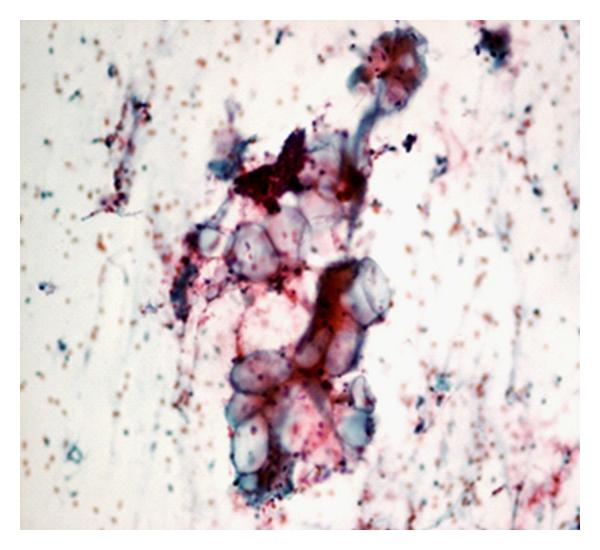
\includegraphics{fig1.jpg}
\caption{image of a fine needle aspirate (FNA) of a breast mass}
\end{figure}

\(~\) \(~\)

Ten real-valued features are computed for each cell nucleus:

\begin{longtable}[]{@{}lrc@{}}
\toprule
Name of the variables & type & Description \\
\midrule
\endhead
1) `radius' & num & distances from center to points on the perimeter \\
2) `texture' & num & standard deviation of gray-scale values \\
3) `perimeter' & num & perimeter of the nucleus \\
4) `area' & num & area of the nucleus \\
5) `smoothness' & num & local variation in radius lengths \\
6) `compactness' & num & \(perimeter^2 / area - 1.0\) \\
7) `concavity' & num & severity of concave portions of the contour \\
8) `concave.points' & num & number of concave portions of the contour \\
9) `symmetry' & num & symmetry of the nucleus \\
10)`fractal\_dimension' & num & \(coastline approximation - 1\) \\
\bottomrule
\end{longtable}

The mean, standard error and ``worst'' or largest (mean of the three
largest values) of these features were computed for each image,
resulting in 30 features. All feature values are recorded with four
significant digits.

The aim is to \textbf{predict whether the cancer is benign or malignant}

\hypertarget{preprocessing}{%
\section{Preprocessing}\label{preprocessing}}

Load data

\begin{Shaded}
\begin{Highlighting}[]
\CommentTok{\#get relative path}
\NormalTok{path }\OtherTok{=} \FunctionTok{here}\NormalTok{(}\StringTok{"LUCILE"}\NormalTok{)}
\FunctionTok{setwd}\NormalTok{(path) }\CommentTok{\#set working directory}

\CommentTok{\# df\textless{}{-}read.csv(\textquotesingle{}/Users/lucile/Library/Mobile Documents/com\textasciitilde{}apple\textasciitilde{}CloudDocs/STUDY/NEURO/LECTURES/stat/data.csv\textquotesingle{},stringsAsFactors = 1)}

\NormalTok{df}\OtherTok{\textless{}{-}}\FunctionTok{read.csv}\NormalTok{(}\StringTok{\textquotesingle{}data.csv\textquotesingle{}}\NormalTok{, }\AttributeTok{stringsAsFactors =} \DecValTok{1}\NormalTok{) }\CommentTok{\# j\textquotesingle{}ai  ajouté le dataset sur github}
\end{Highlighting}
\end{Shaded}

\hypertarget{first-look-into-the-data}{%
\subsection{First look into the data}\label{first-look-into-the-data}}

There are a lot of variables, we should pick the most relevant ones.

Let's delete the last variable and ID number because there are not
relevant.

\begin{Shaded}
\begin{Highlighting}[]
\NormalTok{df}\OtherTok{\textless{}{-}}\NormalTok{df[,}\SpecialCharTok{{-}}\DecValTok{33}\NormalTok{]}
\NormalTok{df}\OtherTok{\textless{}{-}}\NormalTok{df[,}\SpecialCharTok{{-}}\DecValTok{1}\NormalTok{]}
\end{Highlighting}
\end{Shaded}

Let's create a new frame for a the variables of type mean.

\begin{verbatim}
'data.frame':   569 obs. of  11 variables:
 $ diagnosis        : Factor w/ 2 levels "B","M": 2 2 2 2 2 2 2 2 2 2 ...
 $ radius           : num  18 20.6 19.7 11.4 20.3 ...
 $ texture          : num  10.4 17.8 21.2 20.4 14.3 ...
 $ perimeter        : num  122.8 132.9 130 77.6 135.1 ...
 $ area             : num  1001 1326 1203 386 1297 ...
 $ smoothness       : num  0.1184 0.0847 0.1096 0.1425 0.1003 ...
 $ compactness      : num  0.2776 0.0786 0.1599 0.2839 0.1328 ...
 $ concavity        : num  0.3001 0.0869 0.1974 0.2414 0.198 ...
 $ concave.points   : num  0.1471 0.0702 0.1279 0.1052 0.1043 ...
 $ symmetry         : num  0.242 0.181 0.207 0.26 0.181 ...
 $ fractal_dimension: num  0.0787 0.0567 0.06 0.0974 0.0588 ...
\end{verbatim}

\begin{table}
\centering
\resizebox{\linewidth}{!}{
\begin{tabular}{lrrrrrrrrrr}
\toprule
diagnosis & radius & texture & perimeter & area & smoothness & compactness & concavity & concave.points & symmetry & fractal\_dimension\\
\midrule
\cellcolor{gray!6}{M} & \cellcolor{gray!6}{17.99} & \cellcolor{gray!6}{10.38} & \cellcolor{gray!6}{122.80} & \cellcolor{gray!6}{1001.0} & \cellcolor{gray!6}{0.11840} & \cellcolor{gray!6}{0.27760} & \cellcolor{gray!6}{0.3001} & \cellcolor{gray!6}{0.14710} & \cellcolor{gray!6}{0.2419} & \cellcolor{gray!6}{0.07871}\\
M & 20.57 & 17.77 & 132.90 & 1326.0 & 0.08474 & 0.07864 & 0.0869 & 0.07017 & 0.1812 & 0.05667\\
\cellcolor{gray!6}{M} & \cellcolor{gray!6}{19.69} & \cellcolor{gray!6}{21.25} & \cellcolor{gray!6}{130.00} & \cellcolor{gray!6}{1203.0} & \cellcolor{gray!6}{0.10960} & \cellcolor{gray!6}{0.15990} & \cellcolor{gray!6}{0.1974} & \cellcolor{gray!6}{0.12790} & \cellcolor{gray!6}{0.2069} & \cellcolor{gray!6}{0.05999}\\
M & 11.42 & 20.38 & 77.58 & 386.1 & 0.14250 & 0.28390 & 0.2414 & 0.10520 & 0.2597 & 0.09744\\
\cellcolor{gray!6}{M} & \cellcolor{gray!6}{20.29} & \cellcolor{gray!6}{14.34} & \cellcolor{gray!6}{135.10} & \cellcolor{gray!6}{1297.0} & \cellcolor{gray!6}{0.10030} & \cellcolor{gray!6}{0.13280} & \cellcolor{gray!6}{0.1980} & \cellcolor{gray!6}{0.10430} & \cellcolor{gray!6}{0.1809} & \cellcolor{gray!6}{0.05883}\\
\addlinespace
M & 12.45 & 15.70 & 82.57 & 477.1 & 0.12780 & 0.17000 & 0.1578 & 0.08089 & 0.2087 & 0.07613\\
\bottomrule
\end{tabular}}
\end{table}

\begin{verbatim}
 diagnosis     radius          texture        perimeter           area       
 B:357     Min.   : 6.981   Min.   : 9.71   Min.   : 43.79   Min.   : 143.5  
 M:212     1st Qu.:11.700   1st Qu.:16.17   1st Qu.: 75.17   1st Qu.: 420.3  
           Median :13.370   Median :18.84   Median : 86.24   Median : 551.1  
           Mean   :14.127   Mean   :19.29   Mean   : 91.97   Mean   : 654.9  
           3rd Qu.:15.780   3rd Qu.:21.80   3rd Qu.:104.10   3rd Qu.: 782.7  
           Max.   :28.110   Max.   :39.28   Max.   :188.50   Max.   :2501.0  
   smoothness       compactness        concavity       concave.points   
 Min.   :0.05263   Min.   :0.01938   Min.   :0.00000   Min.   :0.00000  
 1st Qu.:0.08637   1st Qu.:0.06492   1st Qu.:0.02956   1st Qu.:0.02031  
 Median :0.09587   Median :0.09263   Median :0.06154   Median :0.03350  
 Mean   :0.09636   Mean   :0.10434   Mean   :0.08880   Mean   :0.04892  
 3rd Qu.:0.10530   3rd Qu.:0.13040   3rd Qu.:0.13070   3rd Qu.:0.07400  
 Max.   :0.16340   Max.   :0.34540   Max.   :0.42680   Max.   :0.20120  
    symmetry      fractal_dimension
 Min.   :0.1060   Min.   :0.04996  
 1st Qu.:0.1619   1st Qu.:0.05770  
 Median :0.1792   Median :0.06154  
 Mean   :0.1812   Mean   :0.06280  
 3rd Qu.:0.1957   3rd Qu.:0.06612  
 Max.   :0.3040   Max.   :0.09744  
\end{verbatim}

Proportion of benign vs malignant cancer

\begin{Shaded}
\begin{Highlighting}[]
\FunctionTok{prop.table}\NormalTok{(}\FunctionTok{table}\NormalTok{(df\_mean}\SpecialCharTok{$}\NormalTok{diagnosis))   }
\end{Highlighting}
\end{Shaded}

\begin{verbatim}
        B         M 
0.6274165 0.3725835 
\end{verbatim}

The two types of cancer are not represented in the same proportion, this
can lead to a bias. Is this proportion representative of the reality ?

``The benign to malignant ratio (B:M ratio) among breast biopsies
(number of benign breast lesions divided by number of breast cancers) is
widely believed to be around 4:1 or 5:1'' {[}2{]}

Blabla citation in parentesis (James 1890) blbabla, or citation in text
James (1890)

\hypertarget{selection-of-variables-of-interest}{%
\subsection{Selection of variables of
interest}\label{selection-of-variables-of-interest}}

According to the description of the data, some variables are likely to
be correlated. We will address this correlation with the mean group of
variable.

Hypothesis about the correlation between variables : \emph{radius and
smoothness should be correlated }radius, perimeter, area and compactness
should be perfectly correlated since it exists a formula between these
variables * concavity and symmetry should be correlated * texture and
fractal\_dimension should not have any correlation

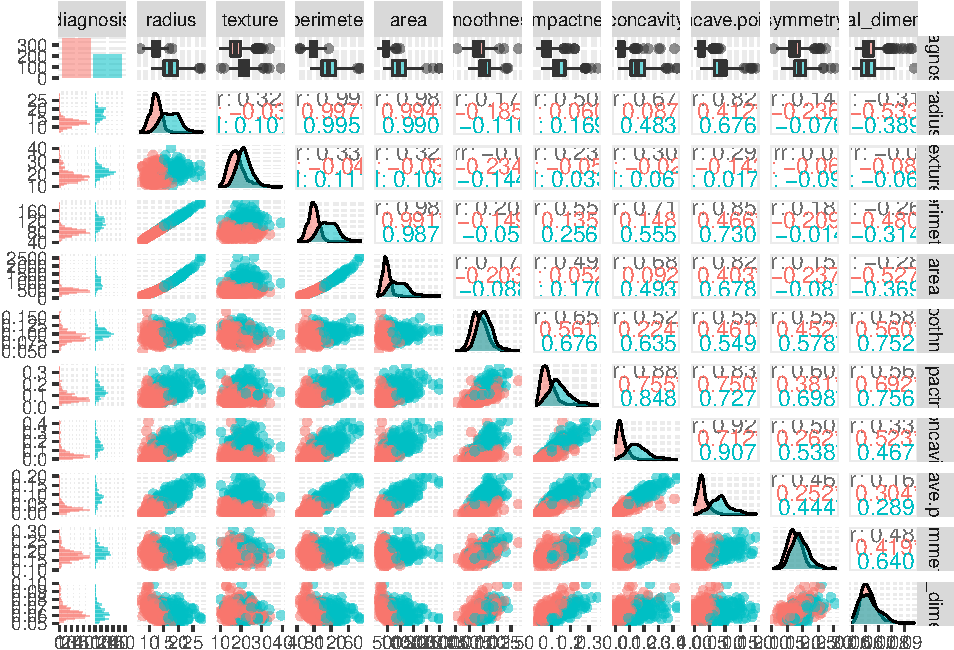
\includegraphics{stat_DAP_files/figure-latex/unnamed-chunk-6-1.pdf}

\begin{verbatim}
## [1] "B" "M"
\end{verbatim}

By eye, the variables seem to be different according to the type of
`diagnosis' (first row of the plot), the variables coming from malignant
cancer seem to be in general bigger than the data coming from bening
cancer.

As expected, radius, perimeter and area are highly correlated;\\
and texture and fractal\_dimension don't have strong correlation.

Surprisingly, radius and smoothness are not very correlated, and the
compactness doesn't show any strong correlation.

Concavity and compactness have a strong correlation. In annexe we show
that we have the same correlations with the standard deviation group and
extreme group of variable.

The following function permit to see better the correlation :

\begin{Shaded}
\begin{Highlighting}[]
\FunctionTok{ggcorr}\NormalTok{(df\_mean, }\AttributeTok{geom =} \StringTok{"text"}\NormalTok{, }\AttributeTok{nbreaks =} \DecValTok{5}\NormalTok{, }\AttributeTok{hjust =} \DecValTok{1}\NormalTok{, }\AttributeTok{label =} \ConstantTok{TRUE}\NormalTok{, }\AttributeTok{label\_alpha =} \FloatTok{0.5}\NormalTok{)}
\end{Highlighting}
\end{Shaded}

\begin{verbatim}
## Warning in ggcorr(df_mean, geom = "text", nbreaks = 5, hjust = 1, label =
## TRUE, : data in column(s) 'diagnosis' are not numeric and were ignored
\end{verbatim}

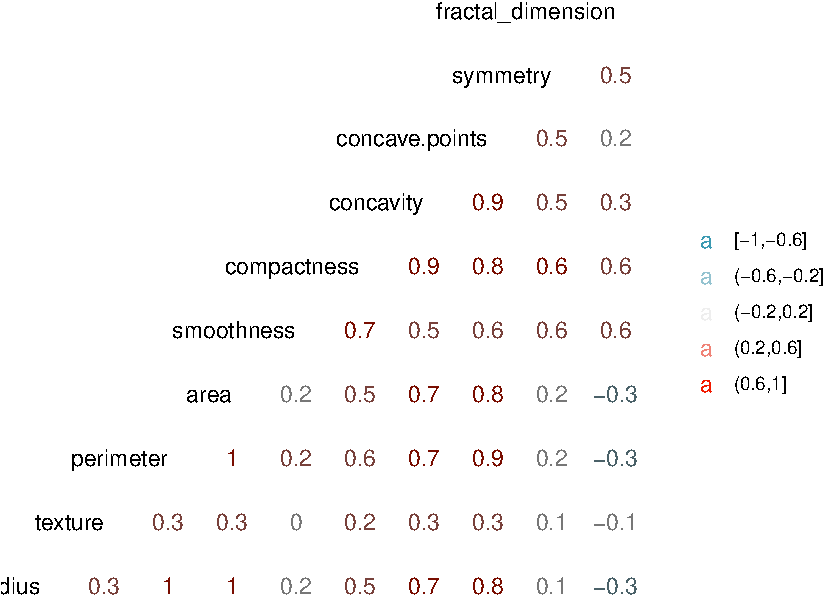
\includegraphics{stat_DAP_files/figure-latex/unnamed-chunk-7-1.pdf} Even
if compactness is define as \(perimeter^2 / area - 1.0\) the correlation
between this variable and area or perimeter is not 1 because the
correlation show only the linear dependency. The correlation between
radius perimeter and area is 1. We will only keep radius.

From here let's remove area, perimeter and compactness

\begin{Shaded}
\begin{Highlighting}[]
\NormalTok{m\_perimeter }\OtherTok{\textless{}{-}}\FunctionTok{lm}\NormalTok{(}\AttributeTok{data =}\NormalTok{ df\_mean,perimeter}\SpecialCharTok{\textasciitilde{}}\NormalTok{ radius}\SpecialCharTok{+}\NormalTok{texture}\SpecialCharTok{+}\NormalTok{area}\SpecialCharTok{+}\NormalTok{smoothness}\SpecialCharTok{+}\NormalTok{compactness}\SpecialCharTok{+}\NormalTok{concavity}\SpecialCharTok{+}\NormalTok{concave.points}\SpecialCharTok{+}\NormalTok{symmetry}\SpecialCharTok{+}\NormalTok{fractal\_dimension)}
\FunctionTok{summary}\NormalTok{(m\_perimeter)}
\end{Highlighting}
\end{Shaded}

\begin{verbatim}
## 
## Call:
## lm(formula = perimeter ~ radius + texture + area + smoothness + 
##     compactness + concavity + concave.points + symmetry + fractal_dimension, 
##     data = df_mean)
## 
## Residuals:
##     Min      1Q  Median      3Q     Max 
## -2.7781 -0.1859  0.0416  0.2280  3.8482 
## 
## Coefficients:
##                     Estimate Std. Error t value Pr(>|t|)    
## (Intercept)        2.627e+00  8.317e-01   3.159  0.00167 ** 
## radius             6.126e+00  5.223e-02 117.301  < 2e-16 ***
## texture           -2.105e-03  5.886e-03  -0.358  0.72073    
## area               3.868e-03  4.676e-04   8.272 9.65e-16 ***
## smoothness        -8.998e+00  2.816e+00  -3.196  0.00147 ** 
## compactness        3.407e+01  1.517e+00  22.459  < 2e-16 ***
## concavity          3.865e+00  9.842e-01   3.927 9.67e-05 ***
## concave.points     4.283e+00  2.785e+00   1.538  0.12456    
## symmetry          -1.930e+00  1.127e+00  -1.712  0.08751 .  
## fractal_dimension -4.119e+01  8.190e+00  -5.029 6.64e-07 ***
## ---
## Signif. codes:  0 '***' 0.001 '**' 0.01 '*' 0.05 '.' 0.1 ' ' 1
## 
## Residual standard error: 0.5538 on 559 degrees of freedom
## Multiple R-squared:  0.9995, Adjusted R-squared:  0.9995 
## F-statistic: 1.214e+05 on 9 and 559 DF,  p-value: < 2.2e-16
\end{verbatim}

\begin{Shaded}
\begin{Highlighting}[]
\NormalTok{m\_area }\OtherTok{\textless{}{-}}\FunctionTok{lm}\NormalTok{(}\AttributeTok{data =}\NormalTok{ df\_mean,area}\SpecialCharTok{\textasciitilde{}}\NormalTok{ radius}\SpecialCharTok{+}\NormalTok{texture}\SpecialCharTok{+}\NormalTok{ perimeter}\SpecialCharTok{+}\NormalTok{smoothness}\SpecialCharTok{+}\NormalTok{compactness}\SpecialCharTok{+}\NormalTok{concavity}\SpecialCharTok{+}\NormalTok{concave.points}\SpecialCharTok{+}\NormalTok{symmetry}\SpecialCharTok{+}\NormalTok{fractal\_dimension)}
\FunctionTok{summary}\NormalTok{(m\_area)}
\end{Highlighting}
\end{Shaded}

\begin{verbatim}
## 
## Call:
## lm(formula = area ~ radius + texture + perimeter + smoothness + 
##     compactness + concavity + concave.points + symmetry + fractal_dimension, 
##     data = df_mean)
## 
## Residuals:
##     Min      1Q  Median      3Q     Max 
## -119.45  -25.53   -8.03   18.13  395.17 
## 
## Coefficients:
##                     Estimate Std. Error t value Pr(>|t|)    
## (Intercept)       -1033.1844    56.7713 -18.199  < 2e-16 ***
## radius              -81.3418    22.3034  -3.647  0.00029 ***
## texture               0.4089     0.5023   0.814  0.41588    
## perimeter            28.1972     3.4086   8.272 9.65e-16 ***
## smoothness           92.0982   242.5499   0.380  0.70431    
## compactness       -2169.2200   153.3091 -14.149  < 2e-16 ***
## concavity           221.0651    84.6672   2.611  0.00927 ** 
## concave.points      295.3508   237.9177   1.241  0.21498    
## symmetry             92.1348    96.4335   0.955  0.33978    
## fractal_dimension  6413.4180   661.4625   9.696  < 2e-16 ***
## ---
## Signif. codes:  0 '***' 0.001 '**' 0.01 '*' 0.05 '.' 0.1 ' ' 1
## 
## Residual standard error: 47.28 on 559 degrees of freedom
## Multiple R-squared:  0.9822, Adjusted R-squared:  0.9819 
## F-statistic:  3434 on 9 and 559 DF,  p-value: < 2.2e-16
\end{verbatim}

\begin{Shaded}
\begin{Highlighting}[]
\NormalTok{m\_compactness }\OtherTok{\textless{}{-}}\FunctionTok{lm}\NormalTok{(}\AttributeTok{data =}\NormalTok{ df\_mean, compactness}\SpecialCharTok{\textasciitilde{}}\NormalTok{ radius}\SpecialCharTok{+}\NormalTok{texture}\SpecialCharTok{+}\NormalTok{ perimeter}\SpecialCharTok{+}\NormalTok{smoothness}\SpecialCharTok{+}\NormalTok{area}\SpecialCharTok{+}\NormalTok{concavity}\SpecialCharTok{+}\NormalTok{concave.points}\SpecialCharTok{+}\NormalTok{symmetry}\SpecialCharTok{+}\NormalTok{fractal\_dimension)}
\FunctionTok{summary}\NormalTok{(m\_compactness)}
\end{Highlighting}
\end{Shaded}

\begin{verbatim}
## 
## Call:
## lm(formula = compactness ~ radius + texture + perimeter + smoothness + 
##     area + concavity + concave.points + symmetry + fractal_dimension, 
##     data = df_mean)
## 
## Residuals:
##       Min        1Q    Median        3Q       Max 
## -0.044976 -0.006177 -0.000675  0.005421  0.058426 
## 
## Coefficients:
##                     Estimate Std. Error t value Pr(>|t|)    
## (Intercept)       -2.053e-01  1.457e-02 -14.091  < 2e-16 ***
## radius            -7.702e-02  4.234e-03 -18.189  < 2e-16 ***
## texture            2.376e-04  1.185e-04   2.004  0.04555 *  
## perimeter          1.392e-02  6.198e-04  22.459  < 2e-16 ***
## smoothness         1.759e-01  5.694e-02   3.089  0.00211 ** 
## area              -1.216e-04  8.592e-06 -14.149  < 2e-16 ***
## concavity          6.410e-02  1.998e-02   3.208  0.00141 ** 
## concave.points     1.077e-01  5.622e-02   1.915  0.05598 .  
## symmetry           9.448e-02  2.250e-02   4.200  3.1e-05 ***
## fractal_dimension  2.348e+00  1.370e-01  17.136  < 2e-16 ***
## ---
## Signif. codes:  0 '***' 0.001 '**' 0.01 '*' 0.05 '.' 0.1 ' ' 1
## 
## Residual standard error: 0.01119 on 559 degrees of freedom
## Multiple R-squared:  0.9558, Adjusted R-squared:  0.9551 
## F-statistic:  1343 on 9 and 559 DF,  p-value: < 2.2e-16
\end{verbatim}

The variables area, perimeter and compactness are well explained by the
other variables ( Adjusted R-squared very close to 1). So we discard
them.

\begin{Shaded}
\begin{Highlighting}[]
\NormalTok{df\_mean\_reduc }\OtherTok{\textless{}{-}}\NormalTok{df\_mean[}\SpecialCharTok{{-}}\FunctionTok{c}\NormalTok{(}\DecValTok{4}\NormalTok{,}\DecValTok{5}\NormalTok{,}\DecValTok{7}\NormalTok{)]}
\end{Highlighting}
\end{Shaded}

\hypertarget{glm}{%
\section{GLM}\label{glm}}

\begin{Shaded}
\begin{Highlighting}[]
\NormalTok{m }\OtherTok{\textless{}{-}}\FunctionTok{glm}\NormalTok{(}\AttributeTok{data =}\NormalTok{ df\_mean, diagnosis}\SpecialCharTok{\textasciitilde{}}\NormalTok{ radius}\SpecialCharTok{+}\NormalTok{texture}\SpecialCharTok{+}\NormalTok{smoothness}\SpecialCharTok{+}\NormalTok{concavity}\SpecialCharTok{+}\NormalTok{concave.points}\SpecialCharTok{+}\NormalTok{symmetry}\SpecialCharTok{+}\NormalTok{fractal\_dimension,}\AttributeTok{family=}\NormalTok{binomial)}
\FunctionTok{summary}\NormalTok{(m)}
\end{Highlighting}
\end{Shaded}

\begin{verbatim}
## 
## Call:
## glm(formula = diagnosis ~ radius + texture + smoothness + concavity + 
##     concave.points + symmetry + fractal_dimension, family = binomial, 
##     data = df_mean)
## 
## Deviance Residuals: 
##      Min        1Q    Median        3Q       Max  
## -2.35180  -0.13938  -0.03229   0.02046   3.15368  
## 
## Coefficients:
##                     Estimate Std. Error z value Pr(>|z|)    
## (Intercept)        -28.38387    6.66946  -4.256 2.08e-05 ***
## radius               0.88701    0.21852   4.059 4.93e-05 ***
## texture              0.37262    0.06212   5.998 2.00e-09 ***
## smoothness          78.50170   32.64920   2.404   0.0162 *  
## concavity           15.52082    8.35462   1.858   0.0632 .  
## concave.points      46.67203   26.16265   1.784   0.0744 .  
## symmetry            16.85783   10.75613   1.567   0.1170    
## fractal_dimension -101.54448   61.26233  -1.658   0.0974 .  
## ---
## Signif. codes:  0 '***' 0.001 '**' 0.01 '*' 0.05 '.' 0.1 ' ' 1
## 
## (Dispersion parameter for binomial family taken to be 1)
## 
##     Null deviance: 751.44  on 568  degrees of freedom
## Residual deviance: 153.35  on 561  degrees of freedom
## AIC: 169.35
## 
## Number of Fisher Scoring iterations: 8
\end{verbatim}

\hypertarget{validation}{%
\subsection{Validation}\label{validation}}

\begin{Shaded}
\begin{Highlighting}[]
\FloatTok{751.44}\SpecialCharTok{/}\FloatTok{153.35}
\end{Highlighting}
\end{Shaded}

\begin{verbatim}
## [1] 4.900163
\end{verbatim}

Overdistribution ?

\begin{Shaded}
\begin{Highlighting}[]
  \FunctionTok{library}\NormalTok{(boot)}
\NormalTok{  diag }\OtherTok{\textless{}{-}} \FunctionTok{glm.diag}\NormalTok{(m)}
  \FunctionTok{glm.diag.plots}\NormalTok{(m, diag)}
\end{Highlighting}
\end{Shaded}

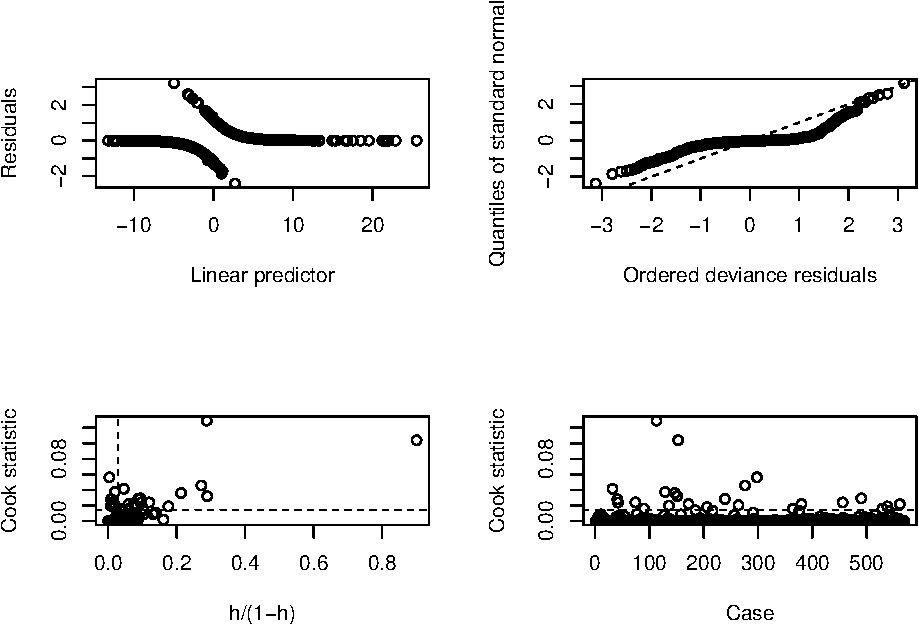
\includegraphics{stat_DAP_files/figure-latex/unnamed-chunk-14-1.pdf}

Let's see with an anova test if we can remove
symmetry,concavity,concave.points and fractal\_dimension

\begin{Shaded}
\begin{Highlighting}[]
\NormalTok{m1 }\OtherTok{\textless{}{-}}\FunctionTok{glm}\NormalTok{(}\AttributeTok{data =}\NormalTok{ df\_mean, diagnosis}\SpecialCharTok{\textasciitilde{}}\NormalTok{ radius}\SpecialCharTok{+}\NormalTok{texture}\SpecialCharTok{+}\NormalTok{smoothness}\SpecialCharTok{+}\NormalTok{concavity}\SpecialCharTok{+}\NormalTok{concave.points}\SpecialCharTok{+}\NormalTok{fractal\_dimension,}\AttributeTok{family=}\NormalTok{binomial)}
\FunctionTok{summary}\NormalTok{(m1)}
\end{Highlighting}
\end{Shaded}

\begin{verbatim}
## 
## Call:
## glm(formula = diagnosis ~ radius + texture + smoothness + concavity + 
##     concave.points + fractal_dimension, family = binomial, data = df_mean)
## 
## Deviance Residuals: 
##      Min        1Q    Median        3Q       Max  
## -2.33122  -0.15084  -0.03480   0.02274   3.04740  
## 
## Coefficients:
##                    Estimate Std. Error z value Pr(>|z|)    
## (Intercept)       -26.65706    6.59839  -4.040 5.35e-05 ***
## radius              0.86784    0.22209   3.908 9.32e-05 ***
## texture             0.36277    0.06098   5.949 2.70e-09 ***
## smoothness         90.53604   33.17393   2.729  0.00635 ** 
## concavity          17.34487    8.23293   2.107  0.03514 *  
## concave.points     45.65526   26.56395   1.719  0.08567 .  
## fractal_dimension -93.18039   59.52661  -1.565  0.11750    
## ---
## Signif. codes:  0 '***' 0.001 '**' 0.01 '*' 0.05 '.' 0.1 ' ' 1
## 
## (Dispersion parameter for binomial family taken to be 1)
## 
##     Null deviance: 751.44  on 568  degrees of freedom
## Residual deviance: 155.78  on 562  degrees of freedom
## AIC: 169.78
## 
## Number of Fisher Scoring iterations: 8
\end{verbatim}

\begin{Shaded}
\begin{Highlighting}[]
\FunctionTok{anova}\NormalTok{(m,m1,}\AttributeTok{test=}\StringTok{"Chisq"}\NormalTok{)}
\end{Highlighting}
\end{Shaded}

\begin{tabular}{r|r|r|r|r}
\hline
Resid. Df & Resid. Dev & Df & Deviance & Pr(>Chi)\\
\hline
561 & 153.3485 & NA & NA & NA\\
\hline
562 & 155.7755 & -1 & -2.426971 & 0.1192631\\
\hline
\end{tabular}

\begin{Shaded}
\begin{Highlighting}[]
\NormalTok{m2 }\OtherTok{\textless{}{-}}\FunctionTok{glm}\NormalTok{(}\AttributeTok{data =}\NormalTok{ df\_mean, diagnosis}\SpecialCharTok{\textasciitilde{}}\NormalTok{ radius}\SpecialCharTok{+}\NormalTok{texture}\SpecialCharTok{+}\NormalTok{smoothness}\SpecialCharTok{+}\NormalTok{concavity}\SpecialCharTok{+}\NormalTok{concave.points,}\AttributeTok{family=}\NormalTok{binomial)}
\FunctionTok{summary}\NormalTok{(m2)}
\end{Highlighting}
\end{Shaded}

\begin{verbatim}
## 
## Call:
## glm(formula = diagnosis ~ radius + texture + smoothness + concavity + 
##     concave.points, family = binomial, data = df_mean)
## 
## Deviance Residuals: 
##      Min        1Q    Median        3Q       Max  
## -2.28927  -0.15267  -0.03761   0.02390   3.03440  
## 
## Coefficients:
##                 Estimate Std. Error z value Pr(>|z|)    
## (Intercept)    -32.18048    5.69324  -5.652 1.58e-08 ***
## radius           0.99766    0.20762   4.805 1.55e-06 ***
## texture          0.36496    0.06131   5.953 2.64e-09 ***
## smoothness      72.72278   30.46830   2.387   0.0170 *  
## concavity       10.21913    6.99120   1.462   0.1438    
## concave.points  48.66262   26.54605   1.833   0.0668 .  
## ---
## Signif. codes:  0 '***' 0.001 '**' 0.01 '*' 0.05 '.' 0.1 ' ' 1
## 
## (Dispersion parameter for binomial family taken to be 1)
## 
##     Null deviance: 751.44  on 568  degrees of freedom
## Residual deviance: 158.34  on 563  degrees of freedom
## AIC: 170.34
## 
## Number of Fisher Scoring iterations: 8
\end{verbatim}

\begin{Shaded}
\begin{Highlighting}[]
\FunctionTok{anova}\NormalTok{(m1,m2,}\AttributeTok{test=}\StringTok{"Chisq"}\NormalTok{)}
\end{Highlighting}
\end{Shaded}

\begin{tabular}{r|r|r|r|r}
\hline
Resid. Df & Resid. Dev & Df & Deviance & Pr(>Chi)\\
\hline
562 & 155.7755 & NA & NA & NA\\
\hline
563 & 158.3372 & -1 & -2.56172 & 0.1094794\\
\hline
\end{tabular}

\begin{Shaded}
\begin{Highlighting}[]
\NormalTok{m3 }\OtherTok{\textless{}{-}}\FunctionTok{glm}\NormalTok{(}\AttributeTok{data =}\NormalTok{ df\_mean, diagnosis}\SpecialCharTok{\textasciitilde{}}\NormalTok{ radius}\SpecialCharTok{+}\NormalTok{texture}\SpecialCharTok{+}\NormalTok{smoothness}\SpecialCharTok{+}\NormalTok{concave.points,}\AttributeTok{family=}\NormalTok{binomial)}
\FunctionTok{summary}\NormalTok{(m3)}
\end{Highlighting}
\end{Shaded}

\begin{verbatim}
## 
## Call:
## glm(formula = diagnosis ~ radius + texture + smoothness + concave.points, 
##     family = binomial, data = df_mean)
## 
## Deviance Residuals: 
##      Min        1Q    Median        3Q       Max  
## -2.42132  -0.15010  -0.04247   0.02603   2.86598  
## 
## Coefficients:
##                 Estimate Std. Error z value Pr(>|z|)    
## (Intercept)    -28.57552    4.81406  -5.936 2.92e-09 ***
## radius           0.85081    0.17112   4.972 6.63e-07 ***
## texture          0.35845    0.05985   5.990 2.10e-09 ***
## smoothness      52.26403   26.08496   2.004   0.0451 *  
## concave.points  78.73692   16.59332   4.745 2.08e-06 ***
## ---
## Signif. codes:  0 '***' 0.001 '**' 0.01 '*' 0.05 '.' 0.1 ' ' 1
## 
## (Dispersion parameter for binomial family taken to be 1)
## 
##     Null deviance: 751.44  on 568  degrees of freedom
## Residual deviance: 160.32  on 564  degrees of freedom
## AIC: 170.32
## 
## Number of Fisher Scoring iterations: 8
\end{verbatim}

\begin{Shaded}
\begin{Highlighting}[]
\FunctionTok{anova}\NormalTok{(m2,m3,}\AttributeTok{test=}\StringTok{"Chisq"}\NormalTok{)}
\end{Highlighting}
\end{Shaded}

\begin{tabular}{r|r|r|r|r}
\hline
Resid. Df & Resid. Dev & Df & Deviance & Pr(>Chi)\\
\hline
563 & 158.3372 & NA & NA & NA\\
\hline
564 & 160.3203 & -1 & -1.983059 & 0.1590686\\
\hline
\end{tabular}

\hypertarget{visualization}{%
\subsection{Visualization}\label{visualization}}

( to see) \#\# glm with glmnet Let's separate the dataset into train and
test set

\begin{Shaded}
\begin{Highlighting}[]
\DocumentationTok{\#\# 75\% of the sample size}
\NormalTok{prop\_train\_test }\OtherTok{\textless{}{-}} \FunctionTok{floor}\NormalTok{(}\FloatTok{0.75} \SpecialCharTok{*} \FunctionTok{nrow}\NormalTok{(df\_mean))}

\DocumentationTok{\#\# set the seed to make your partition reproducible}
\FunctionTok{set.seed}\NormalTok{(}\DecValTok{123}\NormalTok{)}
\NormalTok{train\_ind }\OtherTok{\textless{}{-}} \FunctionTok{sample}\NormalTok{(}\FunctionTok{seq\_len}\NormalTok{(}\FunctionTok{nrow}\NormalTok{(df\_mean)), }\AttributeTok{size =}\NormalTok{ prop\_train\_test)}
\CommentTok{\#sample = sample.split(data$num, SplitRatio = .75)}
\CommentTok{\#train = subset(data, sample == TRUE)}
\CommentTok{\#test  = subset(data, sample == FALSE)}
\NormalTok{train }\OtherTok{\textless{}{-}}\NormalTok{ df\_mean[train\_ind, ]}
\NormalTok{test }\OtherTok{\textless{}{-}}\NormalTok{ df\_mean[}\SpecialCharTok{{-}}\NormalTok{train\_ind, ]}

\NormalTok{x\_train }\OtherTok{\textless{}{-}}\NormalTok{ train[,}\SpecialCharTok{{-}}\DecValTok{1}\NormalTok{]}
\NormalTok{y\_train }\OtherTok{\textless{}{-}}\NormalTok{ train}\SpecialCharTok{$}\NormalTok{diagnosis}
\NormalTok{x\_test }\OtherTok{\textless{}{-}}\NormalTok{  test[,}\SpecialCharTok{{-}}\DecValTok{1}\NormalTok{]}
\NormalTok{y\_test }\OtherTok{\textless{}{-}}\NormalTok{ test}\SpecialCharTok{$}\NormalTok{diagnosis}
\end{Highlighting}
\end{Shaded}

\begin{Shaded}
\begin{Highlighting}[]
\NormalTok{tol\_length}\OtherTok{=}\FunctionTok{length}\NormalTok{(}\FunctionTok{levels}\NormalTok{(y\_train))}

\CommentTok{\# run glm : train and test with cross validation}
\NormalTok{cvfit}\OtherTok{\textless{}{-}}\FunctionTok{cv.glmnet}\NormalTok{(}\FunctionTok{as.matrix}\NormalTok{(x\_train), y\_train,}\AttributeTok{family =} \StringTok{"binomial"}\NormalTok{, }\AttributeTok{type.measure=}\StringTok{"class"}\NormalTok{)}
\FunctionTok{plot}\NormalTok{(cvfit)}
\end{Highlighting}
\end{Shaded}

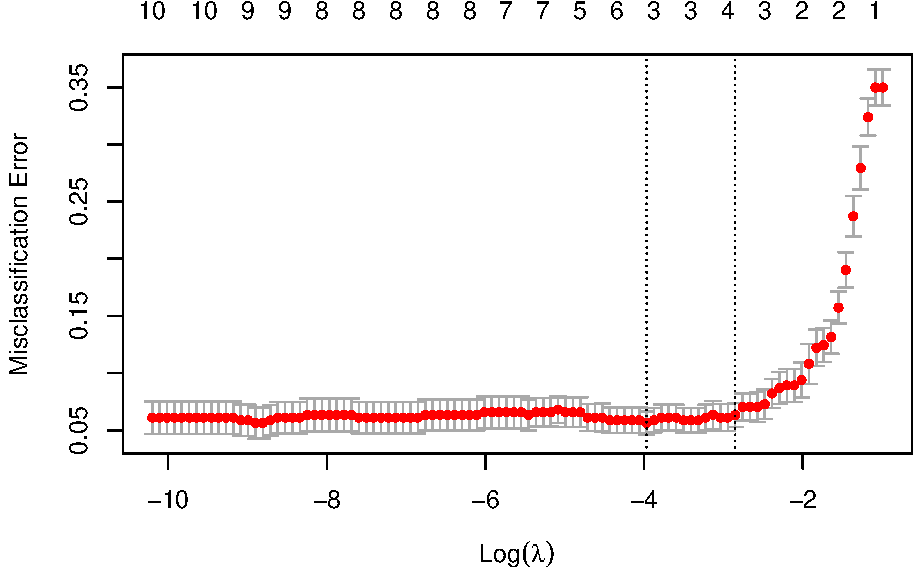
\includegraphics{stat_DAP_files/figure-latex/unnamed-chunk-17-1.pdf}

\begin{Shaded}
\begin{Highlighting}[]
\NormalTok{cvfit}\SpecialCharTok{$}\NormalTok{lambda.min}
\end{Highlighting}
\end{Shaded}

\begin{verbatim}
## [1] 0.01890567
\end{verbatim}

\begin{Shaded}
\begin{Highlighting}[]
\NormalTok{assess}\OtherTok{\textless{}{-}}\FunctionTok{assess.glmnet}\NormalTok{(cvfit,}\AttributeTok{newx=}\FunctionTok{as.matrix}\NormalTok{(x\_test), }\AttributeTok{newy=}\NormalTok{y\_test, }\AttributeTok{s=}\StringTok{\textquotesingle{}lambda.min\textquotesingle{}}\NormalTok{)}
\FunctionTok{confusion.glmnet}\NormalTok{(cvfit, }\AttributeTok{newx =}\FunctionTok{as.matrix}\NormalTok{(x\_test), }\AttributeTok{newy =}\NormalTok{ y\_test, }\AttributeTok{s =} \StringTok{\textquotesingle{}lambda.min\textquotesingle{}}\NormalTok{)}
\end{Highlighting}
\end{Shaded}

\begin{verbatim}
##          True
## Predicted  B  M Total
##     B     79 11    90
##     M      1 52    53
##     Total 80 63   143
## 
##  Percent Correct:  0.9161
\end{verbatim}

\begin{Shaded}
\begin{Highlighting}[]
\FunctionTok{as.numeric}\NormalTok{(}\DecValTok{1}\SpecialCharTok{{-}}\NormalTok{assess}\SpecialCharTok{$}\NormalTok{class)}
\end{Highlighting}
\end{Shaded}

\begin{verbatim}
## [1] 0.9160839
\end{verbatim}

\begin{Shaded}
\begin{Highlighting}[]
\FunctionTok{coef}\NormalTok{(cvfit, }\AttributeTok{s=}\StringTok{"lambda.min"}\NormalTok{)}
\end{Highlighting}
\end{Shaded}

\begin{verbatim}
## 11 x 1 sparse Matrix of class "dgCMatrix"
##                            s1
## (Intercept)       -11.9549638
## radius              0.3363175
## texture             0.1750409
## perimeter           .        
## area                .        
## smoothness          .        
## compactness         .        
## concavity           .        
## concave.points     63.6306102
## symmetry            .        
## fractal_dimension   .
\end{verbatim}

Let's look with the first lambda:

\begin{Shaded}
\begin{Highlighting}[]
\NormalTok{cvfit}\SpecialCharTok{$}\NormalTok{lambda}\FloatTok{.1}\NormalTok{se}
\end{Highlighting}
\end{Shaded}

\begin{verbatim}
## [1] 0.05773519
\end{verbatim}

\begin{Shaded}
\begin{Highlighting}[]
\NormalTok{assess}\OtherTok{\textless{}{-}}\FunctionTok{assess.glmnet}\NormalTok{(cvfit,}\AttributeTok{newx=}\FunctionTok{as.matrix}\NormalTok{(x\_test), }\AttributeTok{newy=}\NormalTok{y\_test, }\AttributeTok{s=}\StringTok{\textquotesingle{}lambda.1se\textquotesingle{}}\NormalTok{)}
\FunctionTok{confusion.glmnet}\NormalTok{(cvfit, }\AttributeTok{newx =}\FunctionTok{as.matrix}\NormalTok{(x\_test), }\AttributeTok{newy =}\NormalTok{ y\_test, }\AttributeTok{s =} \StringTok{\textquotesingle{}lambda.1se\textquotesingle{}}\NormalTok{)}
\end{Highlighting}
\end{Shaded}

\begin{verbatim}
##          True
## Predicted  B  M Total
##     B     80 13    93
##     M      0 50    50
##     Total 80 63   143
## 
##  Percent Correct:  0.9091
\end{verbatim}

\begin{Shaded}
\begin{Highlighting}[]
\FunctionTok{as.numeric}\NormalTok{(}\DecValTok{1}\SpecialCharTok{{-}}\NormalTok{assess}\SpecialCharTok{$}\NormalTok{class)}
\end{Highlighting}
\end{Shaded}

\begin{verbatim}
## [1] 0.9090909
\end{verbatim}

\begin{Shaded}
\begin{Highlighting}[]
\FunctionTok{coef}\NormalTok{(cvfit, }\AttributeTok{s=}\StringTok{"lambda.1se"}\NormalTok{)}
\end{Highlighting}
\end{Shaded}

\begin{verbatim}
## 11 x 1 sparse Matrix of class "dgCMatrix"
##                            s1
## (Intercept)       -6.87636978
## radius             0.01235359
## texture            0.06882308
## perimeter          0.02960914
## area               .         
## smoothness         .         
## compactness        .         
## concavity          .         
## concave.points    40.52201326
## symmetry           .         
## fractal_dimension  .
\end{verbatim}

\hypertarget{pca}{%
\section{PCA}\label{pca}}

\begin{Shaded}
\begin{Highlighting}[]
\NormalTok{p1 }\OtherTok{\textless{}{-}}\FunctionTok{prcomp}\NormalTok{(df\_mean\_reduc[}\SpecialCharTok{{-}}\DecValTok{1}\NormalTok{])}
\FunctionTok{summary}\NormalTok{(p1)}
\end{Highlighting}
\end{Shaded}

\begin{verbatim}
## Importance of components:
##                           PC1    PC2     PC3     PC4     PC5      PC6      PC7
## Standard deviation     4.6080 3.1126 0.06442 0.02211 0.01231 0.006858 0.003604
## Proportion of Variance 0.6866 0.3133 0.00013 0.00002 0.00000 0.000000 0.000000
## Cumulative Proportion  0.6866 0.9998 0.99998 0.99999 1.00000 1.000000 1.000000
\end{verbatim}

\begin{Shaded}
\begin{Highlighting}[]
\CommentTok{\#str(p1)}
\NormalTok{p1}
\end{Highlighting}
\end{Shaded}

\begin{verbatim}
## Standard deviations (1, .., p=7):
## [1] 4.608016307 3.112559143 0.064418475 0.022112044 0.012308580 0.006858361
## [7] 0.003603551
## 
## Rotation (n x k) = (7 x 7):
##                             PC1           PC2          PC3           PC4
## radius            -0.4865963393  0.8734572836 -0.016247190 -0.0031190341
## texture           -0.8735719432 -0.4866917945 -0.001638412 -0.0004536868
## smoothness        -0.0001358489  0.0008343083  0.138357483 -0.1766861095
## concavity         -0.0086261840  0.0119427069  0.895567786  0.3358335663
## concave.points    -0.0045939326  0.0076849313  0.311838508 -0.0748932182
## symmetry          -0.0006740182  0.0008657321  0.272281127 -0.9218545572
## fractal_dimension  0.0002730890 -0.0005821752  0.084667728 -0.0237293409
##                             PC5           PC6           PC7
## radius             0.0019645044  0.0039955704 -1.689040e-03
## texture           -0.0005006787  0.0001269227 -1.471877e-05
## smoothness        -0.7077017950  0.6470590176  1.735261e-01
## concavity          0.2427338224  0.1491793036  6.150564e-02
## concave.points    -0.5944022366 -0.7373962794  5.449565e-04
## symmetry           0.2750833675 -0.0129430718  1.440754e-02
## fractal_dimension -0.1060635323  0.1229771787 -9.827996e-01
\end{verbatim}

\begin{Shaded}
\begin{Highlighting}[]
\FunctionTok{autoplot}\NormalTok{(p1,}\AttributeTok{x=}\DecValTok{1}\NormalTok{, }\AttributeTok{y=}\DecValTok{2}\NormalTok{,}\AttributeTok{data=}\NormalTok{df\_mean,}\AttributeTok{colour =} \StringTok{"diagnosis"}\NormalTok{, }\AttributeTok{loadings =} \ConstantTok{TRUE}\NormalTok{, }\AttributeTok{loadings.colour =} \StringTok{"blue"}\NormalTok{,}
         \AttributeTok{loadings.label =} \ConstantTok{TRUE}\NormalTok{)}
\end{Highlighting}
\end{Shaded}

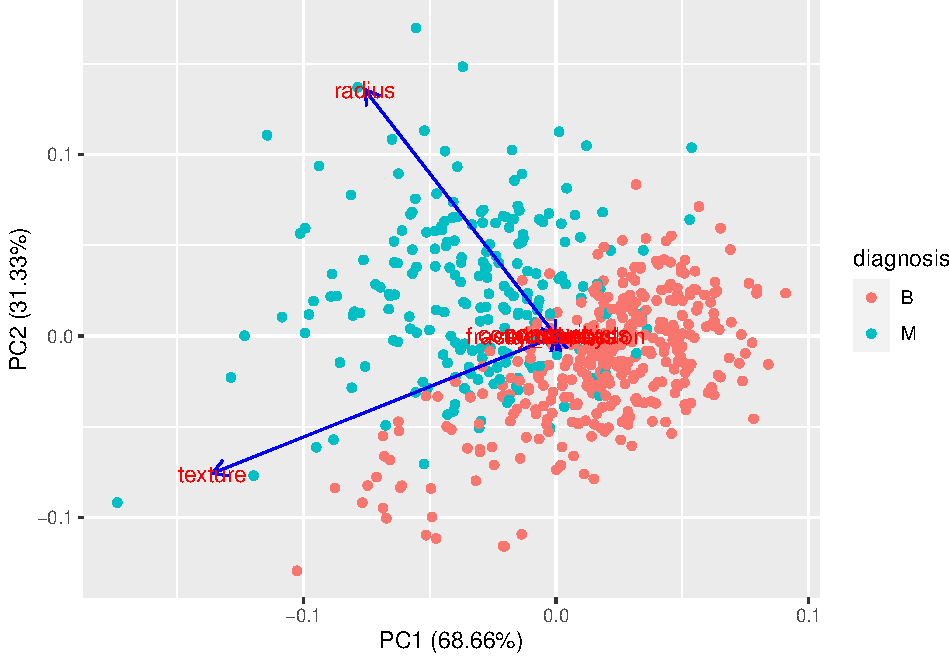
\includegraphics{stat_DAP_files/figure-latex/unnamed-chunk-19-1.pdf}

\begin{Shaded}
\begin{Highlighting}[]
\FunctionTok{autoplot}\NormalTok{(p1,}\AttributeTok{x=}\DecValTok{1}\NormalTok{, }\AttributeTok{y=}\DecValTok{2}\NormalTok{,}\AttributeTok{data=}\NormalTok{df\_mean,}\AttributeTok{colour =} \StringTok{"diagnosis"}\NormalTok{, }\AttributeTok{loadings =} \ConstantTok{TRUE}\NormalTok{, }\AttributeTok{loadings.colour =} \StringTok{"blue"}\NormalTok{,}
         \AttributeTok{loadings.label =} \ConstantTok{TRUE}\NormalTok{)}
\end{Highlighting}
\end{Shaded}

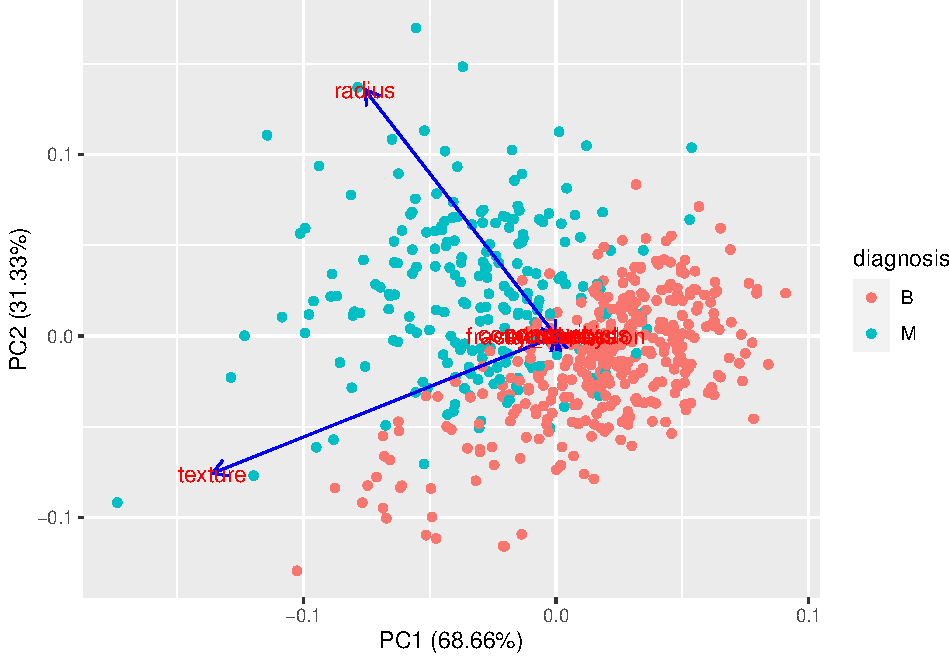
\includegraphics{stat_DAP_files/figure-latex/unnamed-chunk-19-2.pdf} The
first PCA component explain the 99\% of the data. Interpretation
distribution ? k nearst ? pas interpretable

\begin{Shaded}
\begin{Highlighting}[]
\CommentTok{\#install.packages(\textquotesingle{}FNN\textquotesingle{})}
\CommentTok{\#install.packages(\textquotesingle{}crosstable\textquotesingle{})}
\FunctionTok{library}\NormalTok{(crosstable)}
\FunctionTok{library}\NormalTok{(}\StringTok{\textquotesingle{}FNN\textquotesingle{}}\NormalTok{)}
\NormalTok{dat\_pred }\OtherTok{\textless{}{-}}\NormalTok{ FNN }\SpecialCharTok{::} \FunctionTok{knn}\NormalTok{(}\AttributeTok{train =}\NormalTok{x\_train,}\AttributeTok{test=}\NormalTok{  x\_test,}\AttributeTok{cl=}\NormalTok{ y\_train, }\AttributeTok{k =}\DecValTok{10}\NormalTok{)}
\FunctionTok{table}\NormalTok{(}\AttributeTok{x =}\NormalTok{ y\_test, }\AttributeTok{y =}\NormalTok{ dat\_pred)}
\end{Highlighting}
\end{Shaded}

\begin{verbatim}
##    y
## x    B  M
##   B 78  2
##   M 14 49
\end{verbatim}

\begin{Shaded}
\begin{Highlighting}[]
\NormalTok{df\_mean\_pca }\OtherTok{\textless{}{-}} \FunctionTok{cbind}\NormalTok{(df\_mean\_reduc, p1}\SpecialCharTok{$}\NormalTok{x)}
\FunctionTok{summary}\NormalTok{(df\_mean\_pca)}
\end{Highlighting}
\end{Shaded}

\begin{verbatim}
##  diagnosis     radius          texture        smoothness        concavity      
##  B:357     Min.   : 6.981   Min.   : 9.71   Min.   :0.05263   Min.   :0.00000  
##  M:212     1st Qu.:11.700   1st Qu.:16.17   1st Qu.:0.08637   1st Qu.:0.02956  
##            Median :13.370   Median :18.84   Median :0.09587   Median :0.06154  
##            Mean   :14.127   Mean   :19.29   Mean   :0.09636   Mean   :0.08880  
##            3rd Qu.:15.780   3rd Qu.:21.80   3rd Qu.:0.10530   3rd Qu.:0.13070  
##            Max.   :28.110   Max.   :39.28   Max.   :0.16340   Max.   :0.42680  
##  concave.points       symmetry      fractal_dimension      PC1          
##  Min.   :0.00000   Min.   :0.1060   Min.   :0.04996   Min.   :-19.0853  
##  1st Qu.:0.02031   1st Qu.:0.1619   1st Qu.:0.05770   1st Qu.: -3.0771  
##  Median :0.03350   Median :0.1792   Median :0.06154   Median :  0.7017  
##  Mean   :0.04892   Mean   :0.1812   Mean   :0.06280   Mean   :  0.0000  
##  3rd Qu.:0.07400   3rd Qu.:0.1957   3rd Qu.:0.06612   3rd Qu.:  3.3618  
##  Max.   :0.20120   Max.   :0.3040   Max.   :0.09744   Max.   :  9.9883  
##       PC2               PC3                PC4                  PC5            
##  Min.   :-9.6077   Min.   :-0.12749   Min.   :-9.817e-02   Min.   :-0.0501920  
##  1st Qu.:-1.9337   1st Qu.:-0.04061   1st Qu.:-1.222e-02   1st Qu.:-0.0075599  
##  Median :-0.2382   Median :-0.01005   Median :-5.951e-05   Median :-0.0002641  
##  Mean   : 0.0000   Mean   : 0.00000   Mean   : 0.000e+00   Mean   : 0.0000000  
##  3rd Qu.: 1.7827   3rd Qu.: 0.02810   3rd Qu.: 1.368e-02   3rd Qu.: 0.0076599  
##  Max.   :12.6158   Max.   : 0.39962   Max.   : 8.102e-02   Max.   : 0.0632631  
##       PC6                  PC7            
##  Min.   :-3.044e-02   Min.   :-0.0175097  
##  1st Qu.:-4.134e-03   1st Qu.:-0.0017616  
##  Median :-8.956e-05   Median : 0.0002342  
##  Mean   : 0.000e+00   Mean   : 0.0000000  
##  3rd Qu.: 4.320e-03   3rd Qu.: 0.0024175  
##  Max.   : 2.505e-02   Max.   : 0.0108129
\end{verbatim}

\begin{Shaded}
\begin{Highlighting}[]
\NormalTok{glm\_pca }\OtherTok{\textless{}{-}}\FunctionTok{glm}\NormalTok{(}\AttributeTok{data=}\NormalTok{ df\_mean\_pca, df\_mean\_pca}\SpecialCharTok{$}\NormalTok{diagnosis }\SpecialCharTok{\textasciitilde{}}\NormalTok{PC1}\SpecialCharTok{+}\NormalTok{PC2, }\AttributeTok{family =}\NormalTok{ binomial)}
\FunctionTok{summary}\NormalTok{(glm\_pca)}
\end{Highlighting}
\end{Shaded}

\begin{verbatim}
## 
## Call:
## glm(formula = df_mean_pca$diagnosis ~ PC1 + PC2, family = binomial, 
##     data = df_mean_pca)
## 
## Deviance Residuals: 
##     Min       1Q   Median       3Q      Max  
## -2.1460  -0.3791  -0.1203   0.1265   2.8447  
## 
## Coefficients:
##             Estimate Std. Error z value Pr(>|z|)    
## (Intercept) -0.70749    0.15181  -4.660 3.16e-06 ***
## PC1         -0.70531    0.06545 -10.777  < 2e-16 ***
## PC2          0.81767    0.08602   9.506  < 2e-16 ***
## ---
## Signif. codes:  0 '***' 0.001 '**' 0.01 '*' 0.05 '.' 0.1 ' ' 1
## 
## (Dispersion parameter for binomial family taken to be 1)
## 
##     Null deviance: 751.44  on 568  degrees of freedom
## Residual deviance: 290.97  on 566  degrees of freedom
## AIC: 296.97
## 
## Number of Fisher Scoring iterations: 7
\end{verbatim}

\begin{Shaded}
\begin{Highlighting}[]
\FunctionTok{autoplot}\NormalTok{(glm\_pca,}\DecValTok{1}\SpecialCharTok{:}\DecValTok{4}\NormalTok{)}
\end{Highlighting}
\end{Shaded}

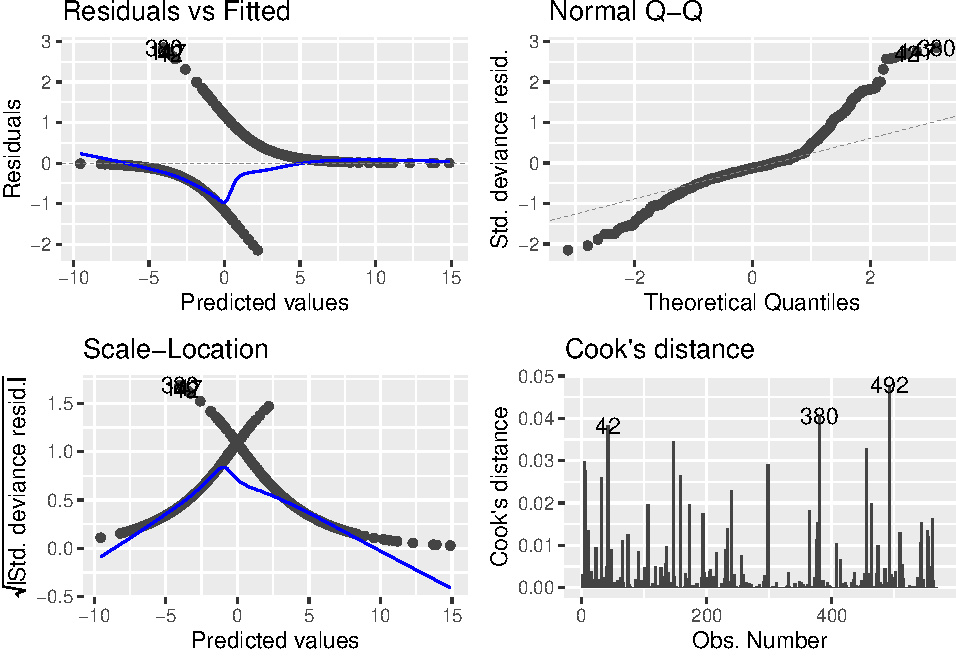
\includegraphics{stat_DAP_files/figure-latex/unnamed-chunk-21-1.pdf}

\begin{Shaded}
\begin{Highlighting}[]
\FunctionTok{ggplot}\NormalTok{(}\AttributeTok{data =}\NormalTok{ df\_mean\_pca, }\FunctionTok{aes}\NormalTok{(}\AttributeTok{x=}\NormalTok{ PC1))}\SpecialCharTok{+} \FunctionTok{geom\_density}\NormalTok{()}
\end{Highlighting}
\end{Shaded}

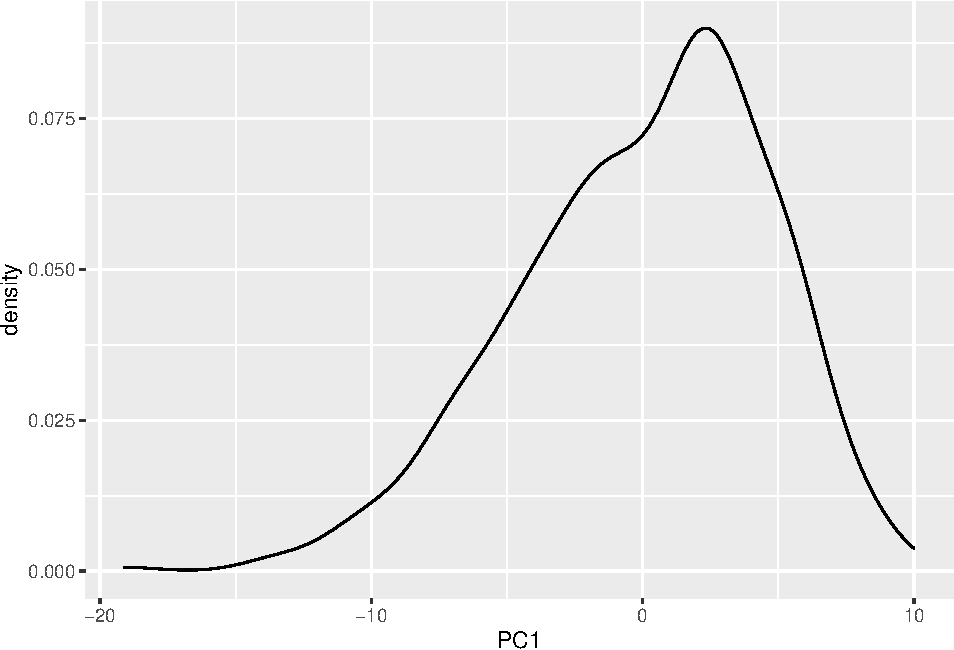
\includegraphics{stat_DAP_files/figure-latex/unnamed-chunk-21-2.pdf}

\begin{Shaded}
\begin{Highlighting}[]
\FunctionTok{ggplot}\NormalTok{(}\AttributeTok{data =}\NormalTok{ df\_mean\_pca, }\FunctionTok{aes}\NormalTok{(}\AttributeTok{x=}\NormalTok{ PC2))}\SpecialCharTok{+} \FunctionTok{geom\_density}\NormalTok{()}
\end{Highlighting}
\end{Shaded}

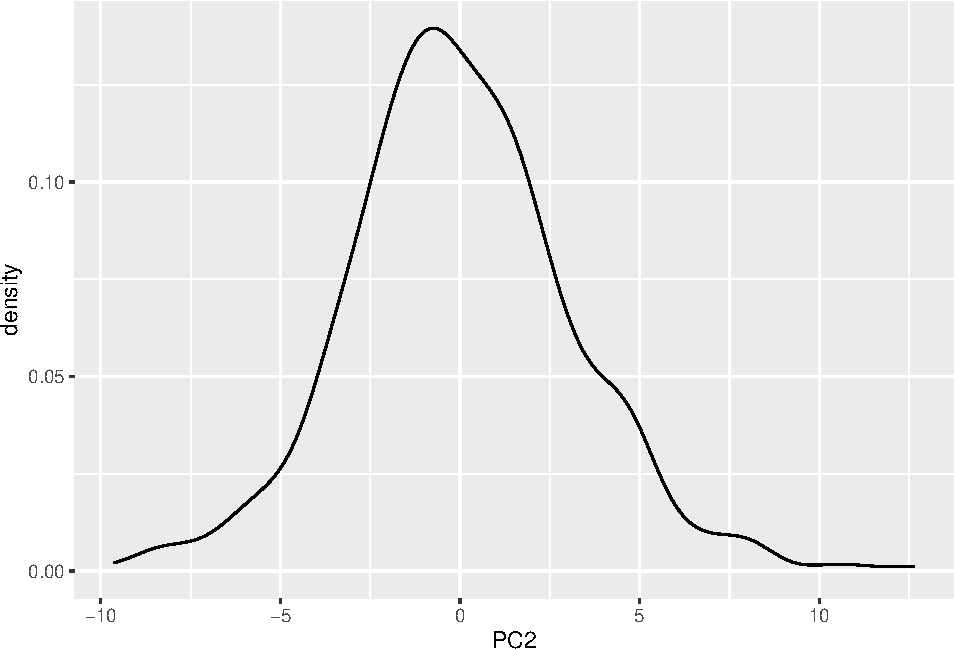
\includegraphics{stat_DAP_files/figure-latex/unnamed-chunk-21-3.pdf}

\begin{center}\rule{0.5\linewidth}{0.5pt}\end{center}

\hypertarget{annexe}{%
\section{Annexe}\label{annexe}}

\hypertarget{more-informations-about-the-dataset}{%
\subsection{More informations about the
dataset}\label{more-informations-about-the-dataset}}

The 3-dimensional space is that described in: {[}3{]}.

This database is also available through the UW CS ftp server: ftp
ftp.cs.wisc.edu cd math-prog/cpo-dataset/machine-learn/WDBC/

\hypertarget{correlation-in-the-standard-deviation-and-worst-group}{%
\subsection{Correlation in the `standard deviation' and `worst'
group}\label{correlation-in-the-standard-deviation-and-worst-group}}

\begin{verbatim}
## 'data.frame':    569 obs. of  11 variables:
##  $ diagnosis         : Factor w/ 2 levels "B","M": 2 2 2 2 2 2 2 2 2 2 ...
##  $ radius            : num  1.095 0.543 0.746 0.496 0.757 ...
##  $ texture           : num  0.905 0.734 0.787 1.156 0.781 ...
##  $ perimeter         : num  8.59 3.4 4.58 3.44 5.44 ...
##  $ area              : num  153.4 74.1 94 27.2 94.4 ...
##  $ smoothness        : num  0.0064 0.00522 0.00615 0.00911 0.01149 ...
##  $ compactness       : num  0.049 0.0131 0.0401 0.0746 0.0246 ...
##  $ concavity         : num  0.0537 0.0186 0.0383 0.0566 0.0569 ...
##  $ concave.points    : num  0.0159 0.0134 0.0206 0.0187 0.0188 ...
##  $ symmetry          : num  0.03 0.0139 0.0225 0.0596 0.0176 ...
##  $ fractal_dimension.: num  0.00619 0.00353 0.00457 0.00921 0.00511 ...
\end{verbatim}

\begin{verbatim}
## `stat_bin()` using `bins = 30`. Pick better value with `binwidth`.
## `stat_bin()` using `bins = 30`. Pick better value with `binwidth`.
## `stat_bin()` using `bins = 30`. Pick better value with `binwidth`.
## `stat_bin()` using `bins = 30`. Pick better value with `binwidth`.
## `stat_bin()` using `bins = 30`. Pick better value with `binwidth`.
## `stat_bin()` using `bins = 30`. Pick better value with `binwidth`.
## `stat_bin()` using `bins = 30`. Pick better value with `binwidth`.
## `stat_bin()` using `bins = 30`. Pick better value with `binwidth`.
## `stat_bin()` using `bins = 30`. Pick better value with `binwidth`.
## `stat_bin()` using `bins = 30`. Pick better value with `binwidth`.
\end{verbatim}

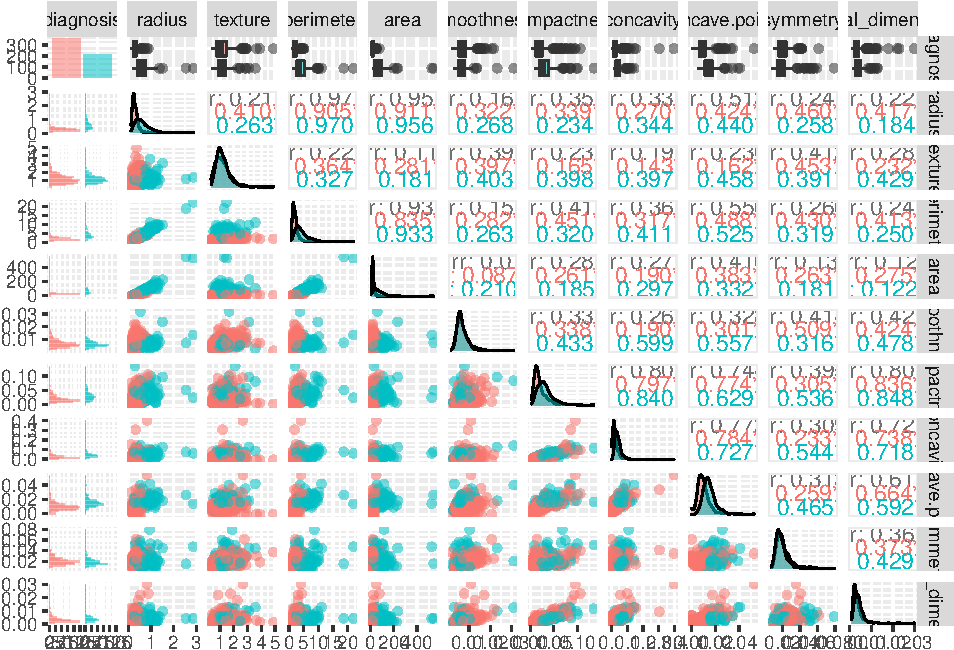
\includegraphics{stat_DAP_files/figure-latex/unnamed-chunk-22-1.pdf}

\begin{verbatim}
## 'data.frame':    569 obs. of  11 variables:
##  $ diagnosis         : Factor w/ 2 levels "B","M": 2 2 2 2 2 2 2 2 2 2 ...
##  $ radius            : num  25.4 25 23.6 14.9 22.5 ...
##  $ texture           : num  17.3 23.4 25.5 26.5 16.7 ...
##  $ perimeter         : num  184.6 158.8 152.5 98.9 152.2 ...
##  $ area              : num  2019 1956 1709 568 1575 ...
##  $ smoothness        : num  0.162 0.124 0.144 0.21 0.137 ...
##  $ compactness       : num  0.666 0.187 0.424 0.866 0.205 ...
##  $ concavity         : num  0.712 0.242 0.45 0.687 0.4 ...
##  $ concave.points    : num  0.265 0.186 0.243 0.258 0.163 ...
##  $ symmetry          : num  0.46 0.275 0.361 0.664 0.236 ...
##  $ fractal_dimension.: num  0.1189 0.089 0.0876 0.173 0.0768 ...
\end{verbatim}

\begin{verbatim}
## `stat_bin()` using `bins = 30`. Pick better value with `binwidth`.
## `stat_bin()` using `bins = 30`. Pick better value with `binwidth`.
## `stat_bin()` using `bins = 30`. Pick better value with `binwidth`.
## `stat_bin()` using `bins = 30`. Pick better value with `binwidth`.
## `stat_bin()` using `bins = 30`. Pick better value with `binwidth`.
## `stat_bin()` using `bins = 30`. Pick better value with `binwidth`.
## `stat_bin()` using `bins = 30`. Pick better value with `binwidth`.
## `stat_bin()` using `bins = 30`. Pick better value with `binwidth`.
## `stat_bin()` using `bins = 30`. Pick better value with `binwidth`.
## `stat_bin()` using `bins = 30`. Pick better value with `binwidth`.
\end{verbatim}

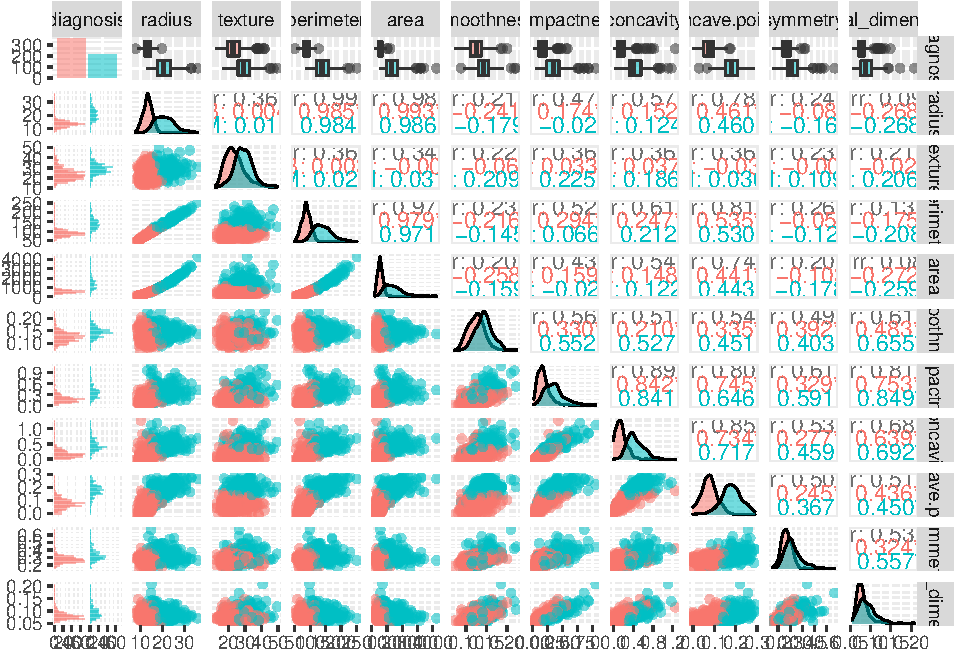
\includegraphics{stat_DAP_files/figure-latex/unnamed-chunk-22-2.pdf}

We get the same results as for the mean group.

\begin{center}\rule{0.5\linewidth}{0.5pt}\end{center}

\hypertarget{references}{%
\section{References}\label{references}}

\begin{itemize}
\tightlist
\item
  {[}1{]}
  \url{https://www.researchgate.net/figure/a-b-Fine-needle-aspiration-cytology-of-the-breast-lesion-showed-singly-lying_fig1_41548857}
\item
  {[}2{]} \url{https://pubmed.ncbi.nlm.nih.gov/7091922/}
\item
  {[}3{]} K. P. Bennett and O. L. Mangasarian: ``Robust Linear
  Programming Discrimination of Two Linearly Inseparable Sets,''
  Optimization Methods and Software 1, 1992, 23-34
\end{itemize}

\hypertarget{version-of-r-used}{%
\section{Version of R used}\label{version-of-r-used}}

\begin{verbatim}
## R version 4.1.1 (2021-08-10)
## Platform: x86_64-apple-darwin17.0 (64-bit)
## Running under: macOS Big Sur 10.16
## 
## Matrix products: default
## BLAS:   /Library/Frameworks/R.framework/Versions/4.1/Resources/lib/libRblas.0.dylib
## LAPACK: /Library/Frameworks/R.framework/Versions/4.1/Resources/lib/libRlapack.dylib
## 
## locale:
## [1] en_US.UTF-8/en_US.UTF-8/en_US.UTF-8/C/en_US.UTF-8/en_US.UTF-8
## 
## attached base packages:
## [1] stats     graphics  grDevices utils     datasets  methods   base     
## 
## other attached packages:
##  [1] FNN_1.1.3         crosstable_0.3.2  boot_1.3-28       glmnet_4.1-3     
##  [5] Matrix_1.3-4      kableExtra_1.3.4  here_1.0.1        MASS_7.3-54      
##  [9] ggfortify_0.4.12  GGally_2.1.2      ggplot2_3.3.5     papaja_0.1.0.9997
## [13] pacman_0.5.1     
## 
## loaded via a namespace (and not attached):
##  [1] Rcpp_1.0.7         svglite_2.0.0      lattice_0.20-44    tidyr_1.1.4       
##  [5] rprojroot_2.0.2    digest_0.6.28      foreach_1.5.1      utf8_1.2.2        
##  [9] R6_2.5.1           plyr_1.8.6         backports_1.2.1    evaluate_0.14     
## [13] httr_1.4.2         highr_0.9          pillar_1.6.3       gdtools_0.2.3     
## [17] rlang_0.4.11       uuid_1.0-3         data.table_1.14.2  rstudioapi_0.13   
## [21] flextable_0.6.10   checkmate_2.0.0    rmarkdown_2.11     labeling_0.4.2    
## [25] splines_4.1.1      webshot_0.5.2      stringr_1.4.0      munsell_0.5.0     
## [29] compiler_4.1.1     xfun_0.26          base64enc_0.1-3    pkgconfig_2.0.3   
## [33] systemfonts_1.0.3  shape_1.4.6        htmltools_0.5.2    tidyselect_1.1.1  
## [37] tibble_3.1.5       gridExtra_2.3      codetools_0.2-18   reshape_0.8.8     
## [41] fansi_0.5.0        viridisLite_0.4.0  crayon_1.4.1       dplyr_1.0.7       
## [45] withr_2.4.2        grid_4.1.1         gtable_0.3.0       lifecycle_1.0.1   
## [49] magrittr_2.0.1     scales_1.1.1       zip_2.2.0          stringi_1.7.5     
## [53] farver_2.1.0       xml2_1.3.3         ellipsis_0.3.2     generics_0.1.0    
## [57] vctrs_0.3.8        RColorBrewer_1.1-2 forcats_0.5.1      iterators_1.0.13  
## [61] tools_4.1.1        glue_1.4.2         officer_0.4.1      purrr_0.3.4       
## [65] fastmap_1.1.0      survival_3.2-11    yaml_2.2.1         colorspace_2.0-2  
## [69] rvest_1.0.2        knitr_1.36
\end{verbatim}

\hypertarget{references-1}{%
\section{References}\label{references-1}}

\(~\) \(~\)

\hypertarget{refs}{}
\begin{CSLReferences}{1}{0}
\leavevmode\vadjust pre{\hypertarget{ref-james_1890}{}}%
James, William. 1890. {``The Perception of Reality.''} \emph{Principles
of Psychology} 2: 283--324.

\end{CSLReferences}

\end{document}
